\documentclass[10pt,a4paper]{article}
\usepackage[UTF8,fontset = none]{ctex}
\setCJKmainfont[BoldFont=黑体,ItalicFont=楷体]{华文中宋}
\usepackage{amssymb,amsmath,amsfonts,amsthm,mathrsfs,dsfont,graphicx}
\usepackage{ifthen,indentfirst,enumerate,color,titletoc}
\usepackage{tikz}
\usepackage{multicol}
\usepackage{makecell}
\usepackage{longtable}
\usetikzlibrary{arrows,calc,intersections,patterns,decorations.pathreplacing,3d,angles,quotes}
\usepackage[bf,small,indentafter,pagestyles]{titlesec}
\usepackage[top=1in, bottom=1in,left=0.8in,right=0.8in]{geometry}
\renewcommand{\baselinestretch}{1.65}
\newtheorem{defi}{定义~}
\newtheorem{eg}{例~}
\newtheorem{ex}{~}
\newtheorem{rem}{注~}
\newtheorem{thm}{定理~}
\newtheorem{coro}{推论~}
\newtheorem{axiom}{公理~}
\newtheorem{prop}{性质~}
\newcommand{\blank}[1]{\underline{\hbox to #1pt{}}}
\newcommand{\bracket}[1]{(\hbox to #1pt{})}
\newcommand{\onech}[4]{\par\begin{tabular}{p{.9\textwidth}}
A.~#1\\
B.~#2\\
C.~#3\\
D.~#4
\end{tabular}}
\newcommand{\twoch}[4]{\par\begin{tabular}{p{.46\textwidth}p{.46\textwidth}}
A.~#1& B.~#2\\
C.~#3& D.~#4
\end{tabular}}
\newcommand{\vartwoch}[4]{\par\begin{tabular}{p{.46\textwidth}p{.46\textwidth}}
(1)~#1& (2)~#2\\
(3)~#3& (4)~#4
\end{tabular}}
\newcommand{\fourch}[4]{\par\begin{tabular}{p{.23\textwidth}p{.23\textwidth}p{.23\textwidth}p{.23\textwidth}}
A.~#1 &B.~#2& C.~#3& D.~#4
\end{tabular}}
\newcommand{\varfourch}[4]{\par\begin{tabular}{p{.23\textwidth}p{.23\textwidth}p{.23\textwidth}p{.23\textwidth}}
(1)~#1 &(2)~#2& (3)~#3& (4)~#4
\end{tabular}}
\begin{document}

\begin{enumerate}[1.]
\item 判断下列命题是否正确:\\
(1) 终边重合的两个角相等;\\
(2) 锐角是第一象限的角;\\
(3) 第二象限的角是钝角;\\
(4) 小于$90^\circ$的角都是锐角.
\item 分别用集合的形式表示终边位于第三象限的所有角和终边位于$y$轴正半轴上的所有角.
\item 在$0^\circ-360^\circ$范围内, 分别找出终边与下列各角的终边重合的角, 并判断它们是第几象限的角:\\
(1) $-315^\circ$\\
(2) $905.3^\circ$;\\
(3) $-1090^\circ$;\\
(4) $530^\circ$.
\item 分别将下列角度化为弧度:\\
(1) $15^\circ$;\\
(2) $-108^\circ$;\\
(3) $22^\circ 30'$.
\item 分别将下列弧度化为角度:
(1) $\dfrac{11}{12}\pi$;\\
(2) $-\dfrac 25\pi$;\\
(3) $-3$(结果精确到$0.01^\circ$).
\item 已知扇形的弧所对的圆心角为$54^\circ$, 且半径为$10\text{cm}$. 求该扇形的弧长和面积.
\item 如果$\alpha$是第三象限的角, 判断$\dfrac\alpha 2$是哪个象限的角.
\item 已知角$\alpha$的终边过点$P(2a, -3a)$($a<0$), 求角$\alpha$的正弦、余弦、正切及余切值.
\item 已知角$\alpha$的终边过点$P(0, -3)$, 则下列值不存在的是\bracket{20}.
\fourch{$\sin \alpha$}{$\cos \alpha$}{$\tan \alpha$}{$\cot \alpha$}
\item 根据下列条件, 分别判断角$\theta$属于第几象限:\\
(1) $\sin \theta =-\dfrac 12$且$\cos \theta =-\dfrac{\sqrt 3}2$;\\
(2) $\sin \theta <0$且$\tan \theta >0$.
\item 求角$\dfrac 53\pi$的正弦、余弦、正切及余切值.
\item 分别求$\sin k\pi$($k\in \mathbf{Z}$)和$\cos k\pi$($k\in \mathbf{Z}$)的值.
\item 已知$\alpha$为第三象限的角, $\cos \alpha=-\dfrac{\sqrt 5}5$. 求$\sin \alpha$、$\tan \alpha$及$\cot \alpha$.
\item 已知$\cot \alpha=\dfrac 13$, 求$\sin \alpha$、$\cos \alpha$及$\tan \alpha$.
\item 已知$\tan \alpha=3$, 求$\dfrac{2\sin \alpha+\cos \alpha}{\sin \alpha-\cos \alpha}$的值.
\item 化简:\\
(1) $\sin ^2\alpha+\sin ^2\alpha\cos ^2\alpha+\cos^4\alpha$;\\
(2) $\sin \alpha\cos \alpha(\tan \alpha+\cot \alpha)$.
\item 证明: $\cot ^2\alpha-\cos ^2\alpha=\cot ^2\alpha\cdot \cos ^2\alpha$.
\item 证明:\\
(1) $\sin (2\pi -\alpha)=-\sin \alpha$;\\
(2) $\cos (2\pi -\alpha)=\cos \alpha$;\\
(3) $\tan (2\pi -\alpha)=-\tan \alpha$;\\
(4) $\cot (2\pi -\alpha)=-\cot \alpha$.
\item 利用诱导公式求值:\\
(1) $\sin \dfrac{11}4\pi$;\\
(2) $\cos (-\dfrac 56\pi)$;\\
(3) $\tan (-\dfrac{14}3\pi)$.
\item 化简:\\
(1) $\dfrac{\sin (180^\circ -\alpha)}{\sin (180^\circ +\alpha)}+\dfrac{\cos (360^\circ -\alpha)}{\cos (180^\circ +\alpha)}+\dfrac{\tan (180^\circ +\alpha)}{\tan (-\alpha)}$;\\
(2) $\dfrac{\sin (\pi -\alpha)}{\cos (\pi +\alpha)}\cdot \dfrac{\sin (2\pi -\alpha)}{\tan (\pi +\alpha)}$.
\item 证明:\\
(1) $\sin (\dfrac{3\pi}2-\alpha)=-\cos \alpha$;\\
(2) $\cos (\dfrac{3\pi}2-\alpha)=-\sin \alpha$;\\
(3) $\tan (\dfrac{3\pi}2-\alpha)=\cot \alpha$;\\
(4) $\cot (\dfrac{3\pi}2-\alpha)=\tan \alpha$.
\item 化简: $\dfrac{\sin (\dfrac\pi 2+\alpha)\cot (\dfrac{3\pi}2-\alpha)\cos (3\pi +\alpha)}{\cot (\dfrac\pi 2-\alpha)\cos (\dfrac{3\pi} 2+\alpha)\cot (\pi -\alpha)}$.
\item 已知点$A$的坐标为$(3, 4)$, 将$OA$绕坐标原点$O$顺时针旋转$\dfrac\pi 2$至$OA'$. 求点$A'$的坐标.
\item 根据下列条件, 分别求角$x$:\\
(1) 已知$\sin x=-\dfrac{\sqrt 3}2$;\\
(2) 已知$\cos x=-\dfrac 12$;\\
(3) 已知$\tan x=-\sqrt 3$.
\item 分别求满足下列条件的角$x$的集合:\\
(1) $2\sin (x+\dfrac\pi 3)=1$, $x\in [0, 2\pi ]$;\\
(2) $\cos (2x+\dfrac \pi 4)=-\dfrac 12$;\\
(3) $\tan (3x+\dfrac \pi 4)=-1$.
\item 化简:\\
(1) $\cos (22^\circ -x)\cos (23^\circ +x)-\sin (22^\circ -x)\sin (23^\circ +x)$;\\
(2) $\cos (\dfrac\pi 6+\alpha)\cos \alpha+\sin (\dfrac \pi 6+\alpha)\sin \alpha$.
\item 已知$\sin \theta =-\dfrac 5{13}$, $\theta \in (\pi , \dfrac3 2\pi )$. 求$\cos (\theta +\dfrac \pi 4)$的值.
\item 证明:\\
(1) $\dfrac{2\cos A\cos B-\cos (A-B)}{\cos (A-B)-2\sin A\sin B}=1$;\\
(2) $\cos (\alpha+\beta)\cos (\alpha-\beta)=\cos^2\beta-\sin ^2\alpha$.
\item 求下列各式的值:\\
(1) $\sin \dfrac{5\pi}{12}\cos \dfrac\pi{12}-\cos \dfrac{5\pi}{12}\sin \dfrac\pi {12}$;
(2) $\dfrac{1+\tan 15^\circ}{1-\tan 15^\circ}$.
\item 已知$\cos \theta =-\dfrac 35$, $\theta \in (0, \pi)$. 求$\sin (\theta +\dfrac\pi 4)$和$\tan (\theta -\dfrac\pi 4)$的值.
\item 证明下列恒等式:\\
(1) $\dfrac{\sin (\alpha+\beta)\sin (\alpha-\beta)}{\cos^2\alpha\cos^2\beta}=\tan^2\alpha-\tan^2\beta$;\\
(2) $\tan (\theta +\dfrac\pi 4)=\dfrac{1+\tan \theta}{1-\tan \theta}$.
\item 在$\triangle ABC$中, 已知$\cos A=\dfrac{12}{13}$, $\cos B=\dfrac8{17}$. 求$\sin C$和$\cos C$的值.
\item 已知$\cos \alpha=\dfrac 45$, $\alpha\in (0, \dfrac \pi 2)$, $\sin \beta=\dfrac{12}{13}$, $\beta\in (\dfrac\pi 2, \pi )$. 求$\sin (\alpha+\beta)$和$\cos (\alpha+\beta)$的值, 并判断$\alpha+\beta$是第几象限的角.
\item 把下列各式化为$A\sin (\alpha+\varphi )$($A>0$)的形式:\\
(1) $\sin \alpha+\cos \alpha$;\\
(2) $-\sin \alpha+\sqrt 3\cos \alpha$.
\item 利用二倍角公式, 求下列各式的值:\\
(1) $\sin \dfrac{5\pi}{12}\cos\dfrac{5\pi}{12}$;\\
(2) $\cos^222.5^\circ -\sin^222. 5^\circ$;\\
(3) $\dfrac{\tan 15^\circ}{1-\tan^215^\circ}$.
\item 已知$\cos \alpha=-\dfrac{\sqrt 5}5$, $\alpha\in (\dfrac\pi 2, \pi)$. 求$\sin 2\alpha$, $\cos 2\alpha$和$\tan 2\alpha$的值.
\item 证明下列恒等式:\\
(1) $(\sin \alpha+\cos \alpha)^2=1+\sin 2\alpha$;\\
(2) $\cos^4\alpha-\sin^4\alpha=\cos 2\alpha$;\\
(3) $\sin 3\alpha=3\sin \alpha-4\sin^3\alpha$.
\item 证明: $\cos \alpha\cos \beta=\dfrac 12[\cos (\alpha+\beta)+\cos (\alpha-\beta)]$.
\item 证明: $\cos \alpha+\cos \beta=2\cos \dfrac{\alpha+\beta}
2 \cos \dfrac{\alpha-\beta}2$.
\item 证明: $\tan \dfrac\alpha2=\dfrac{1-\cos \alpha}{\sin \alpha}$.
\item 在$\triangle ABC$中, 已知$a=7$, $B=30^\circ$, $C=85^\circ$. 求$c$. (结果精确到$0. 01$)
\item 在$\triangle ABC$中, 已知$a=5$, $A=40^\circ$, $B=80^\circ$. 求$b$、$c$和面积$S$. (结果精确到$0. 01$)
\item 在$\triangle ABC$中, 如果$\sin^2A+\sin^2B=\sin^2C$, 试判断该三角形的形状. 
练习6. 3(2)
\item 在$\triangle ABC$中, 已知$a=3$, $b=4$, $C=60^\circ$. 求$c$.
\item 在$\triangle ABC$中, 已知$A=45^\circ$, $a=2\sqrt 6$, $b=2\sqrt 3$. 求$B$、$C$及$c$.
\item 在$\triangle ABC$中, 已知三边之比为$2:3:4$. 求该三角形的最大角的余弦值.
\item 在$\triangle ABC$中, 已知$a=4$, $B=60^\circ$, 其面积为$5\sqrt 3$. 求$b$.
\item 证明: 平行四边形中, 四边平方和等于对角线平方和.
\item 在$\triangle ABC$中, 求证:\\
(1) $\dfrac{a^2+b^2}{c^2}=\dfrac{\sin^2A+\sin^2B}{\sin^2C}$;\\
(2) $a^2+b^2+c^2=2(bc\cos A+ac\cos B+ab\cos C)$.
\item 分别求满足下列条件的角.\\
(1) $\sin x=\dfrac 35$, $x\in  [-\dfrac\pi 2, \dfrac\pi 2]$;\\
(2) $\cos x=-\dfrac 23$, $x\in [0, \pi ]$;\\
(3) $\tan x=-2$, $x\in (-\dfrac\pi 2, \dfrac\pi 2)$;\\
(4) $\sin x=-\dfrac 23$, $x\in \mathbf{R}$. 
\item 某货轮在$A$处看灯塔$S$在北偏东$30^\circ$方向. 它以每小时$18$海里的速度向正北方向航行, 经过$40$分钟航行到$B$处, 看灯塔$S$在北偏东$75^\circ$方向. 求此时货轮到灯塔$S$的距离.
\item 我缉私船发现位于正北方向的走私船以每小时$30$海里的速度向北偏东$45^\circ$方向的公海逃窜, 已知缉私船的最大时速是$45$海里, 为了及时截住走私船, 缉私船应以什么方向追击走私船?  (结果精确到$0.01^\circ$)
\item 修建铁路时要在一个山体上开挖一隧道, 需要测量隧道口$D$、$E$之间的距离. 测量人员在山的一侧选取点$C$, 因有障碍物, 无法直接测得$CE$及$DE$的距离. 现测得$CA=482. 80\text{m}$, $CB=631.50\text{m}$, $\angle ACB=56.3^\circ$; 又测得$A$及$B$两点到隧道口的距离分别是$80.13\text{m}$及$40.24\text{m}$($A$、$D$、$E$、$B$在同一直线上). 求隧道
$DE$的长. (结果精确到$1\text{m}$)
\begin{center}
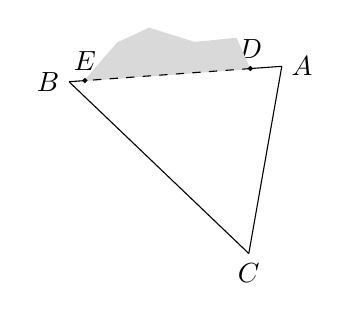
\begin{tikzpicture}[>=latex,scale = 0.5]
\draw (0,0) node [below] {$C$} coordinate (C);
\draw (C) --++ (80:4.828) node [right] {$A$} coordinate (A);
\draw (C) --++ ({80+56.3}:6.315) node [left] {$B$} coordinate (B);
\path [name path = AB] (A) -- (B);
\path [name path = circleA] (A) circle (0.8013);
\path [name path = circleB] (B) circle (0.4024);
\path [name intersections = {of = AB and circleA, by = D}];
\draw (D) node [above] {$D$} -- (A);
\path [name intersections = {of = AB and circleB, by = E}];
\draw (E) node [above] {$E$} -- (B);
\filldraw [gray!30] (D) -- (E) -- ($(E)!0.3!45:(D)$) -- ($(E)!0.5!35:(D)$) -- ($(E)!0.7!15:(D)$) -- ($(D)!0.2!-70:(E)$);
\draw [dashed] (D) -- (E);
\filldraw (D) circle (0.05) (E) circle (0.05);
\end{tikzpicture}
\end{center}
\item 作出函数$y=\sin x$, $x\in [-\pi , \pi ]$的大致图像.
\item 作出函数$y=\dfrac 12-\sin x$, $x\in [0, 2\pi ]$的大致图像, 并分别写出使得$y>0$和$y<0$的$x$的取值范围.
\item 在同一平面直角坐标系中作出$y=\sin x$和$y=\sin x+2$的大致图像, 并说明它们之间的关系.
\item 求下列函数的最小正周期:\\
(1) $y=-\dfrac 13\sin x+1$;\\
(2) $y=3\sin (3x-\dfrac\pi 6)$.
\item 当$x=2k\pi +\dfrac{4\pi} 3$($k\in \mathbf{Z}$)时, $\sin (x+\dfrac\pi 3)=\sin x$是否成立? 如果成立, 那么$\dfrac \pi 3$是不是
$y=\sin x$的周期? 为什么?
\item 现实生活中常碰到类似于周期的现象. 根据图中标出的尺度估算下列心电图的周期. (其中横轴的单位是$2\text{ms}$, $1\text{s}=1000\text{ms}$; 纵轴的单位是$\text{mV}$)
\begin{center}
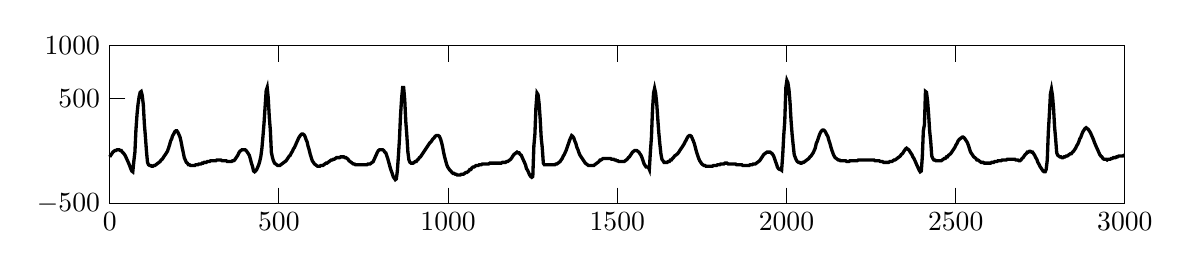
\begin{tikzpicture}[>=latex]
\draw [very thick] (0.000,0.59) -- (0.013,0.61) -- (0.027,0.63) -- (0.040,0.65) -- (0.053,0.66) -- (0.067,0.67) -- (0.080,0.67) -- (0.093,0.68) -- (0.107,0.68) -- (0.120,0.68) -- (0.133,0.67) -- (0.147,0.67) -- (0.160,0.65) -- (0.173,0.64) -- (0.187,0.62) -- (0.200,0.60) -- (0.213,0.57) -- (0.227,0.54) -- (0.240,0.51) -- (0.253,0.48) -- (0.267,0.44) -- (0.280,0.41) -- (0.293,0.40) -- (0.307,0.54) -- (0.320,0.65) -- (0.333,0.93) -- (0.347,1.13) -- (0.360,1.26) -- (0.373,1.35) -- (0.387,1.41) -- (0.400,1.42) -- (0.413,1.37) -- (0.427,1.25) -- (0.440,1.01) -- (0.453,0.85) -- (0.467,0.66) -- (0.480,0.52) -- (0.493,0.49) -- (0.507,0.48) -- (0.520,0.48) -- (0.533,0.47) -- (0.547,0.47) -- (0.560,0.48) -- (0.573,0.48) -- (0.587,0.49) -- (0.600,0.50) -- (0.613,0.51) -- (0.627,0.52) -- (0.640,0.53) -- (0.653,0.55) -- (0.667,0.56) -- (0.680,0.58) -- (0.693,0.60) -- (0.707,0.62) -- (0.720,0.64) -- (0.733,0.66) -- (0.747,0.70) -- (0.760,0.74) -- (0.773,0.79) -- (0.787,0.82) -- (0.800,0.86) -- (0.813,0.88) -- (0.827,0.91) -- (0.840,0.92) -- (0.853,0.92) -- (0.867,0.90) -- (0.880,0.87) -- (0.893,0.84) -- (0.907,0.78) -- (0.920,0.71) -- (0.933,0.65) -- (0.947,0.58) -- (0.960,0.55) -- (0.973,0.52) -- (0.987,0.51) -- (1.000,0.49) -- (1.013,0.49) -- (1.027,0.48) -- (1.040,0.48) -- (1.053,0.48) -- (1.067,0.48) -- (1.080,0.48) -- (1.093,0.49) -- (1.107,0.49) -- (1.120,0.49) -- (1.133,0.50) -- (1.147,0.50) -- (1.160,0.50) -- (1.173,0.51) -- (1.187,0.51) -- (1.200,0.52) -- (1.213,0.52) -- (1.227,0.52) -- (1.240,0.53) -- (1.253,0.53) -- (1.267,0.53) -- (1.280,0.54) -- (1.293,0.54) -- (1.307,0.54) -- (1.320,0.54) -- (1.333,0.54) -- (1.347,0.54) -- (1.360,0.55) -- (1.373,0.55) -- (1.387,0.55) -- (1.400,0.55) -- (1.413,0.55) -- (1.427,0.54) -- (1.440,0.54) -- (1.453,0.54) -- (1.467,0.54) -- (1.480,0.54) -- (1.493,0.53) -- (1.507,0.53) -- (1.520,0.53) -- (1.533,0.53) -- (1.547,0.53) -- (1.560,0.54) -- (1.573,0.54) -- (1.587,0.55) -- (1.600,0.57) -- (1.613,0.59) -- (1.627,0.61) -- (1.640,0.64) -- (1.653,0.66) -- (1.667,0.67) -- (1.680,0.68) -- (1.693,0.68) -- (1.707,0.68) -- (1.720,0.68) -- (1.733,0.67) -- (1.747,0.65) -- (1.760,0.63) -- (1.773,0.61) -- (1.787,0.56) -- (1.800,0.51) -- (1.813,0.47) -- (1.827,0.41) -- (1.840,0.40) -- (1.853,0.41) -- (1.867,0.43) -- (1.880,0.46) -- (1.893,0.49) -- (1.907,0.54) -- (1.920,0.60) -- (1.933,0.70) -- (1.947,0.86) -- (1.960,1.02) -- (1.973,1.22) -- (1.987,1.43) -- (2.000,1.47) -- (2.013,1.34) -- (2.027,1.09) -- (2.040,0.93) -- (2.053,0.65) -- (2.067,0.58) -- (2.080,0.54) -- (2.093,0.51) -- (2.107,0.50) -- (2.120,0.49) -- (2.133,0.48) -- (2.147,0.48) -- (2.160,0.48) -- (2.173,0.49) -- (2.187,0.50) -- (2.200,0.51) -- (2.213,0.52) -- (2.227,0.53) -- (2.240,0.54) -- (2.253,0.56) -- (2.267,0.58) -- (2.280,0.60) -- (2.293,0.61) -- (2.307,0.64) -- (2.320,0.66) -- (2.333,0.69) -- (2.347,0.71) -- (2.360,0.74) -- (2.373,0.77) -- (2.387,0.80) -- (2.400,0.83) -- (2.413,0.85) -- (2.427,0.87) -- (2.440,0.88) -- (2.453,0.88) -- (2.467,0.87) -- (2.480,0.85) -- (2.493,0.81) -- (2.507,0.78) -- (2.520,0.72) -- (2.533,0.68) -- (2.547,0.62) -- (2.560,0.58) -- (2.573,0.54) -- (2.587,0.52) -- (2.600,0.50) -- (2.613,0.49) -- (2.627,0.48) -- (2.640,0.47) -- (2.653,0.47) -- (2.667,0.47) -- (2.680,0.48) -- (2.693,0.48) -- (2.707,0.48) -- (2.720,0.49) -- (2.733,0.50) -- (2.747,0.51) -- (2.760,0.51) -- (2.773,0.52) -- (2.787,0.53) -- (2.800,0.54) -- (2.813,0.55) -- (2.827,0.55) -- (2.840,0.56) -- (2.853,0.56) -- (2.867,0.57) -- (2.880,0.58) -- (2.893,0.58) -- (2.907,0.58) -- (2.920,0.58) -- (2.933,0.59) -- (2.947,0.59) -- (2.960,0.59) -- (2.973,0.59) -- (2.987,0.58) -- (3.000,0.58) -- (3.013,0.57) -- (3.027,0.56) -- (3.040,0.54) -- (3.053,0.53) -- (3.067,0.52) -- (3.080,0.51) -- (3.093,0.50) -- (3.107,0.50) -- (3.120,0.49) -- (3.133,0.49) -- (3.147,0.49) -- (3.160,0.49) -- (3.173,0.49) -- (3.187,0.49) -- (3.200,0.49) -- (3.213,0.49) -- (3.227,0.49) -- (3.240,0.49) -- (3.253,0.49) -- (3.267,0.49) -- (3.280,0.50) -- (3.293,0.50) -- (3.307,0.50) -- (3.320,0.51) -- (3.333,0.52) -- (3.347,0.53) -- (3.360,0.56) -- (3.373,0.59) -- (3.387,0.62) -- (3.400,0.65) -- (3.413,0.67) -- (3.427,0.68) -- (3.440,0.68) -- (3.453,0.68) -- (3.467,0.68) -- (3.480,0.67) -- (3.493,0.65) -- (3.507,0.64) -- (3.520,0.60) -- (3.533,0.56) -- (3.547,0.51) -- (3.560,0.46) -- (3.573,0.42) -- (3.587,0.38) -- (3.600,0.34) -- (3.613,0.32) -- (3.627,0.30) -- (3.640,0.31) -- (3.653,0.41) -- (3.667,0.61) -- (3.680,0.82) -- (3.693,1.11) -- (3.707,1.33) -- (3.720,1.47) -- (3.733,1.47) -- (3.747,1.31) -- (3.760,1.04) -- (3.773,0.87) -- (3.787,0.65) -- (3.800,0.55) -- (3.813,0.52) -- (3.827,0.51) -- (3.840,0.51) -- (3.853,0.51) -- (3.867,0.52) -- (3.880,0.53) -- (3.893,0.53) -- (3.907,0.55) -- (3.920,0.56) -- (3.933,0.58) -- (3.947,0.59) -- (3.960,0.61) -- (3.973,0.63) -- (3.987,0.65) -- (4.000,0.67) -- (4.013,0.69) -- (4.027,0.71) -- (4.040,0.73) -- (4.053,0.75) -- (4.067,0.77) -- (4.080,0.78) -- (4.093,0.80) -- (4.107,0.82) -- (4.120,0.83) -- (4.133,0.85) -- (4.147,0.86) -- (4.160,0.86) -- (4.173,0.86) -- (4.187,0.85) -- (4.200,0.82) -- (4.213,0.78) -- (4.227,0.72) -- (4.240,0.65) -- (4.253,0.59) -- (4.267,0.54) -- (4.280,0.49) -- (4.293,0.46) -- (4.307,0.44) -- (4.320,0.42) -- (4.333,0.41) -- (4.347,0.39) -- (4.360,0.38) -- (4.373,0.38) -- (4.387,0.37) -- (4.400,0.37) -- (4.413,0.36) -- (4.427,0.36) -- (4.440,0.36) -- (4.453,0.36) -- (4.467,0.37) -- (4.480,0.37) -- (4.493,0.37) -- (4.507,0.38) -- (4.520,0.39) -- (4.533,0.39) -- (4.547,0.40) -- (4.560,0.41) -- (4.573,0.43) -- (4.587,0.43) -- (4.600,0.45) -- (4.613,0.46) -- (4.627,0.46) -- (4.640,0.47) -- (4.653,0.48) -- (4.667,0.48) -- (4.680,0.48) -- (4.693,0.49) -- (4.707,0.49) -- (4.720,0.49) -- (4.733,0.50) -- (4.747,0.50) -- (4.760,0.50) -- (4.773,0.50) -- (4.787,0.50) -- (4.800,0.50) -- (4.813,0.50) -- (4.827,0.51) -- (4.840,0.51) -- (4.853,0.51) -- (4.867,0.51) -- (4.880,0.51) -- (4.893,0.51) -- (4.907,0.51) -- (4.920,0.51) -- (4.933,0.51) -- (4.947,0.51) -- (4.960,0.51) -- (4.973,0.51) -- (4.987,0.52) -- (5.000,0.52) -- (5.013,0.52) -- (5.027,0.52) -- (5.040,0.53) -- (5.053,0.53) -- (5.067,0.54) -- (5.080,0.55) -- (5.093,0.56) -- (5.107,0.58) -- (5.120,0.60) -- (5.133,0.62) -- (5.147,0.63) -- (5.160,0.64) -- (5.173,0.65) -- (5.187,0.64) -- (5.200,0.64) -- (5.213,0.62) -- (5.227,0.61) -- (5.240,0.58) -- (5.253,0.55) -- (5.267,0.52) -- (5.280,0.49) -- (5.293,0.44) -- (5.307,0.42) -- (5.320,0.39) -- (5.333,0.36) -- (5.347,0.34) -- (5.360,0.33) -- (5.373,0.34) -- (5.387,0.73) -- (5.400,0.88) -- (5.413,1.22) -- (5.427,1.40) -- (5.440,1.38) -- (5.453,1.27) -- (5.467,1.07) -- (5.480,0.83) -- (5.493,0.71) -- (5.507,0.51) -- (5.520,0.49) -- (5.533,0.49) -- (5.547,0.49) -- (5.560,0.49) -- (5.573,0.49) -- (5.587,0.49) -- (5.600,0.49) -- (5.613,0.49) -- (5.627,0.49) -- (5.640,0.49) -- (5.653,0.49) -- (5.667,0.50) -- (5.680,0.50) -- (5.693,0.51) -- (5.707,0.52) -- (5.720,0.53) -- (5.733,0.55) -- (5.747,0.57) -- (5.760,0.60) -- (5.773,0.62) -- (5.787,0.65) -- (5.800,0.68) -- (5.813,0.72) -- (5.827,0.76) -- (5.840,0.80) -- (5.853,0.83) -- (5.867,0.86) -- (5.880,0.85) -- (5.893,0.83) -- (5.907,0.79) -- (5.920,0.76) -- (5.933,0.71) -- (5.947,0.68) -- (5.960,0.64) -- (5.973,0.61) -- (5.987,0.59) -- (6.000,0.57) -- (6.013,0.55) -- (6.027,0.53) -- (6.040,0.51) -- (6.053,0.50) -- (6.067,0.49) -- (6.080,0.48) -- (6.093,0.48) -- (6.107,0.48) -- (6.120,0.48) -- (6.133,0.48) -- (6.147,0.48) -- (6.160,0.49) -- (6.173,0.50) -- (6.187,0.51) -- (6.200,0.52) -- (6.213,0.53) -- (6.227,0.55) -- (6.240,0.55) -- (6.253,0.56) -- (6.267,0.57) -- (6.280,0.57) -- (6.293,0.57) -- (6.307,0.57) -- (6.320,0.57) -- (6.333,0.57) -- (6.347,0.57) -- (6.360,0.57) -- (6.373,0.56) -- (6.387,0.56) -- (6.400,0.56) -- (6.413,0.55) -- (6.427,0.55) -- (6.440,0.54) -- (6.453,0.54) -- (6.467,0.53) -- (6.480,0.53) -- (6.493,0.53) -- (6.507,0.53) -- (6.520,0.53) -- (6.533,0.53) -- (6.547,0.54) -- (6.560,0.55) -- (6.573,0.56) -- (6.587,0.58) -- (6.600,0.59) -- (6.613,0.61) -- (6.627,0.63) -- (6.640,0.65) -- (6.653,0.66) -- (6.667,0.67) -- (6.680,0.67) -- (6.693,0.67) -- (6.707,0.66) -- (6.720,0.65) -- (6.733,0.63) -- (6.747,0.61) -- (6.760,0.58) -- (6.773,0.54) -- (6.787,0.50) -- (6.800,0.48) -- (6.813,0.46) -- (6.827,0.46) -- (6.840,0.46) -- (6.853,0.43) -- (6.867,0.66) -- (6.880,0.84) -- (6.893,1.18) -- (6.907,1.40) -- (6.920,1.46) -- (6.933,1.40) -- (6.947,1.27) -- (6.960,1.08) -- (6.973,0.90) -- (6.987,0.75) -- (7.000,0.63) -- (7.013,0.56) -- (7.027,0.54) -- (7.040,0.52) -- (7.053,0.52) -- (7.067,0.52) -- (7.080,0.52) -- (7.093,0.53) -- (7.107,0.53) -- (7.120,0.55) -- (7.133,0.55) -- (7.147,0.57) -- (7.160,0.58) -- (7.173,0.60) -- (7.187,0.61) -- (7.200,0.62) -- (7.213,0.63) -- (7.227,0.65) -- (7.240,0.67) -- (7.253,0.69) -- (7.267,0.71) -- (7.280,0.73) -- (7.293,0.75) -- (7.307,0.78) -- (7.320,0.80) -- (7.333,0.83) -- (7.347,0.85) -- (7.360,0.86) -- (7.373,0.86) -- (7.387,0.85) -- (7.400,0.82) -- (7.413,0.79) -- (7.427,0.75) -- (7.440,0.70) -- (7.453,0.65) -- (7.467,0.61) -- (7.480,0.57) -- (7.493,0.54) -- (7.507,0.52) -- (7.520,0.50) -- (7.533,0.49) -- (7.547,0.48) -- (7.560,0.48) -- (7.573,0.47) -- (7.587,0.47) -- (7.600,0.47) -- (7.613,0.47) -- (7.627,0.47) -- (7.640,0.47) -- (7.653,0.47) -- (7.667,0.48) -- (7.680,0.48) -- (7.693,0.48) -- (7.707,0.48) -- (7.720,0.49) -- (7.733,0.49) -- (7.747,0.49) -- (7.760,0.50) -- (7.773,0.50) -- (7.787,0.50) -- (7.800,0.50) -- (7.813,0.51) -- (7.827,0.51) -- (7.840,0.51) -- (7.853,0.50) -- (7.867,0.50) -- (7.880,0.50) -- (7.893,0.50) -- (7.907,0.50) -- (7.920,0.50) -- (7.933,0.50) -- (7.947,0.50) -- (7.960,0.49) -- (7.973,0.49) -- (7.987,0.49) -- (8.000,0.49) -- (8.013,0.49) -- (8.027,0.49) -- (8.040,0.48) -- (8.053,0.48) -- (8.067,0.48) -- (8.080,0.48) -- (8.093,0.48) -- (8.107,0.48) -- (8.120,0.48) -- (8.133,0.49) -- (8.147,0.49) -- (8.160,0.49) -- (8.173,0.50) -- (8.187,0.50) -- (8.200,0.50) -- (8.213,0.51) -- (8.227,0.52) -- (8.240,0.53) -- (8.253,0.54) -- (8.267,0.56) -- (8.280,0.58) -- (8.293,0.60) -- (8.307,0.62) -- (8.320,0.63) -- (8.333,0.64) -- (8.347,0.65) -- (8.360,0.65) -- (8.373,0.65) -- (8.387,0.65) -- (8.400,0.64) -- (8.413,0.63) -- (8.427,0.61) -- (8.440,0.58) -- (8.453,0.54) -- (8.467,0.50) -- (8.480,0.46) -- (8.493,0.44) -- (8.507,0.43) -- (8.520,0.43) -- (8.533,0.42) -- (8.547,0.61) -- (8.560,0.86) -- (8.573,1.04) -- (8.587,1.47) -- (8.600,1.56) -- (8.613,1.53) -- (8.627,1.44) -- (8.640,1.28) -- (8.653,1.05) -- (8.667,0.87) -- (8.680,0.74) -- (8.693,0.62) -- (8.707,0.58) -- (8.720,0.55) -- (8.733,0.53) -- (8.747,0.52) -- (8.760,0.52) -- (8.773,0.51) -- (8.787,0.51) -- (8.800,0.52) -- (8.813,0.52) -- (8.827,0.53) -- (8.840,0.54) -- (8.853,0.55) -- (8.867,0.56) -- (8.880,0.57) -- (8.893,0.59) -- (8.907,0.60) -- (8.920,0.62) -- (8.933,0.64) -- (8.947,0.67) -- (8.960,0.70) -- (8.973,0.76) -- (8.987,0.79) -- (9.000,0.83) -- (9.013,0.87) -- (9.027,0.90) -- (9.040,0.92) -- (9.053,0.93) -- (9.067,0.93) -- (9.080,0.92) -- (9.093,0.90) -- (9.107,0.87) -- (9.120,0.85) -- (9.133,0.80) -- (9.147,0.76) -- (9.160,0.71) -- (9.173,0.67) -- (9.187,0.63) -- (9.200,0.60) -- (9.213,0.58) -- (9.227,0.57) -- (9.240,0.56) -- (9.253,0.55) -- (9.267,0.55) -- (9.280,0.54) -- (9.293,0.54) -- (9.307,0.54) -- (9.320,0.54) -- (9.333,0.54) -- (9.347,0.54) -- (9.360,0.53) -- (9.373,0.53) -- (9.387,0.53) -- (9.400,0.54) -- (9.413,0.54) -- (9.427,0.54) -- (9.440,0.54) -- (9.453,0.54) -- (9.467,0.54) -- (9.480,0.54) -- (9.493,0.54) -- (9.507,0.55) -- (9.520,0.55) -- (9.533,0.55) -- (9.547,0.55) -- (9.560,0.55) -- (9.573,0.55) -- (9.587,0.55) -- (9.600,0.55) -- (9.613,0.55) -- (9.627,0.55) -- (9.640,0.55) -- (9.653,0.55) -- (9.667,0.55) -- (9.680,0.55) -- (9.693,0.55) -- (9.707,0.55) -- (9.720,0.54) -- (9.733,0.54) -- (9.747,0.54) -- (9.760,0.54) -- (9.773,0.54) -- (9.787,0.53) -- (9.800,0.53) -- (9.813,0.53) -- (9.827,0.52) -- (9.840,0.52) -- (9.853,0.52) -- (9.867,0.52) -- (9.880,0.52) -- (9.893,0.52) -- (9.907,0.53) -- (9.920,0.53) -- (9.933,0.53) -- (9.947,0.54) -- (9.960,0.55) -- (9.973,0.55) -- (9.987,0.56) -- (10.000,0.57) -- (10.013,0.58) -- (10.027,0.59) -- (10.040,0.60) -- (10.053,0.62) -- (10.067,0.63) -- (10.080,0.65) -- (10.093,0.67) -- (10.107,0.69) -- (10.120,0.70) -- (10.133,0.69) -- (10.147,0.68) -- (10.160,0.66) -- (10.173,0.64) -- (10.187,0.62) -- (10.200,0.59) -- (10.213,0.57) -- (10.227,0.54) -- (10.240,0.51) -- (10.253,0.48) -- (10.267,0.45) -- (10.280,0.42) -- (10.293,0.40) -- (10.307,0.41) -- (10.320,0.59) -- (10.333,0.92) -- (10.347,1.00) -- (10.360,1.42) -- (10.373,1.41) -- (10.387,1.30) -- (10.400,1.13) -- (10.413,0.92) -- (10.427,0.78) -- (10.440,0.60) -- (10.453,0.57) -- (10.467,0.55) -- (10.480,0.55) -- (10.493,0.54) -- (10.507,0.54) -- (10.520,0.54) -- (10.533,0.54) -- (10.547,0.54) -- (10.560,0.54) -- (10.573,0.55) -- (10.587,0.56) -- (10.600,0.57) -- (10.613,0.57) -- (10.627,0.59) -- (10.640,0.59) -- (10.653,0.61) -- (10.667,0.62) -- (10.680,0.63) -- (10.693,0.65) -- (10.707,0.67) -- (10.720,0.69) -- (10.733,0.71) -- (10.747,0.74) -- (10.760,0.76) -- (10.773,0.79) -- (10.787,0.81) -- (10.800,0.82) -- (10.813,0.83) -- (10.827,0.84) -- (10.840,0.84) -- (10.853,0.83) -- (10.867,0.81) -- (10.880,0.79) -- (10.893,0.77) -- (10.907,0.73) -- (10.920,0.69) -- (10.933,0.65) -- (10.947,0.63) -- (10.960,0.61) -- (10.973,0.59) -- (10.987,0.58) -- (11.000,0.57) -- (11.013,0.55) -- (11.027,0.55) -- (11.040,0.54) -- (11.053,0.53) -- (11.067,0.52) -- (11.080,0.52) -- (11.093,0.52) -- (11.107,0.51) -- (11.120,0.51) -- (11.133,0.51) -- (11.147,0.51) -- (11.160,0.51) -- (11.173,0.51) -- (11.187,0.51) -- (11.200,0.52) -- (11.213,0.52) -- (11.227,0.52) -- (11.240,0.53) -- (11.253,0.53) -- (11.267,0.53) -- (11.280,0.54) -- (11.293,0.54) -- (11.307,0.54) -- (11.320,0.54) -- (11.333,0.55) -- (11.347,0.55) -- (11.360,0.55) -- (11.373,0.55) -- (11.387,0.55) -- (11.400,0.56) -- (11.413,0.56) -- (11.427,0.56) -- (11.440,0.56) -- (11.453,0.56) -- (11.467,0.56) -- (11.480,0.56) -- (11.493,0.56) -- (11.507,0.55) -- (11.520,0.55) -- (11.533,0.55) -- (11.547,0.54) -- (11.560,0.54) -- (11.573,0.55) -- (11.587,0.57) -- (11.600,0.58) -- (11.613,0.60) -- (11.627,0.62) -- (11.640,0.63) -- (11.653,0.65) -- (11.667,0.65) -- (11.680,0.66) -- (11.693,0.66) -- (11.707,0.65) -- (11.720,0.65) -- (11.733,0.63) -- (11.747,0.61) -- (11.760,0.58) -- (11.773,0.56) -- (11.787,0.52) -- (11.800,0.50) -- (11.813,0.47) -- (11.827,0.45) -- (11.840,0.43) -- (11.853,0.41) -- (11.867,0.40) -- (11.880,0.40) -- (11.893,0.43) -- (11.907,0.55) -- (11.920,0.90) -- (11.933,1.12) -- (11.947,1.39) -- (11.960,1.45) -- (11.973,1.37) -- (11.987,1.20) -- (12.000,0.97) -- (12.013,0.82) -- (12.027,0.64) -- (12.040,0.61) -- (12.053,0.60) -- (12.067,0.59) -- (12.080,0.59) -- (12.093,0.58) -- (12.107,0.58) -- (12.120,0.59) -- (12.133,0.59) -- (12.147,0.60) -- (12.160,0.60) -- (12.173,0.61) -- (12.187,0.62) -- (12.200,0.63) -- (12.213,0.63) -- (12.227,0.65) -- (12.240,0.66) -- (12.253,0.68) -- (12.267,0.70) -- (12.280,0.73) -- (12.293,0.75) -- (12.307,0.78) -- (12.320,0.82) -- (12.333,0.84) -- (12.347,0.88) -- (12.360,0.91) -- (12.373,0.93) -- (12.387,0.95) -- (12.400,0.96) -- (12.413,0.95) -- (12.427,0.94) -- (12.440,0.92) -- (12.453,0.90) -- (12.467,0.87) -- (12.480,0.84) -- (12.493,0.81) -- (12.507,0.77) -- (12.520,0.74) -- (12.533,0.71) -- (12.547,0.68) -- (12.560,0.65) -- (12.573,0.62) -- (12.587,0.60) -- (12.600,0.59) -- (12.613,0.57) -- (12.627,0.56) -- (12.640,0.56) -- (12.653,0.56) -- (12.667,0.55) -- (12.680,0.56) -- (12.693,0.56) -- (12.707,0.56) -- (12.720,0.57) -- (12.733,0.57) -- (12.747,0.58) -- (12.760,0.58) -- (12.773,0.58) -- (12.787,0.59) -- (12.800,0.59) -- (12.813,0.60) -- (12.827,0.60) -- (12.840,0.60) -- (12.853,0.60) -- (12.867,0.60) -- (12.880,0.61) -- (12.893,0.61) ;
\draw (0,0) rectangle (12.893,2);
\draw (0,0) node [left] {$-500$} node [below] {$0$};
\draw (0.2,1.333) -- (0,1.333) node [left] {$500$};
\draw (0,2) node [left] {$1000$};
\foreach \i in {500,1000,...,3000}
{\draw (\i/3000*12.893,0.2) -- (\i/3000*12.893,0) node [below] {$\i$};
\draw (\i/3000*12.893,1.8) -- (\i/3000*12.893,2);};
\end{tikzpicture}
\end{center}
\item 求下列函数的定义域和值域:\\
(1) $y=\sin (x+\dfrac \pi 2)$;\\
(2) $y=2\sin x$.
\item 求下列函数的最大值与最小值:\\
(1) $y=-5+\sin (2x+\dfrac \pi 4)$;\\
(2) $y=\cos 2x+2\sin x$;\\
(3) $y=2\sin x\cdot \cos x-\sqrt 3\cos 2x+\sqrt 3\sin 2x$.
\item 如图, 矩形$ABCD$的四个顶点分别在矩形$A_1B_1C_1D_1$的
四条边上, $AB=a$, $BC=b$. 如果$AB$与$A_1B_1$的夹角为$\alpha$, 那
么当$\alpha$取何值时, 矩形$A_1B_1C_1D_1$的周长最大?
\begin{center}
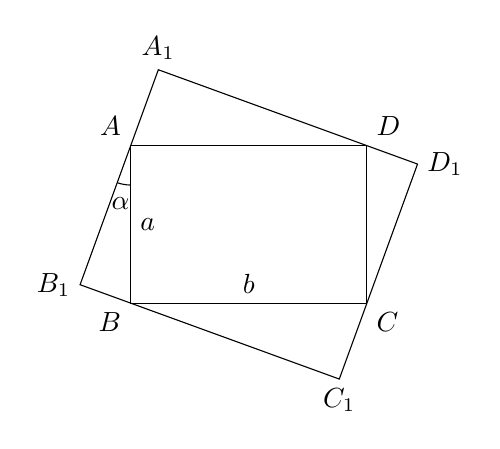
\begin{tikzpicture}[>=latex]
\draw (0,0) node [below left] {$B$} coordinate (B) -- (3,0) node [below right] {$C$} coordinate (C) -- (3,2) node [above right] {$D$} coordinate (D) -- (0,2) node [above left] {$A$} coordinate (A) -- cycle;
\draw (A) --++ (70:{3*cos(70)}) node [above] {$A_1$} -- (D);
\draw (D) --++ (-20:{2*cos(70)}) node [right] {$D_1$} -- (C);
\draw (C) --++ (-110:{3*cos(70)}) node [below] {$C_1$} -- (B);
\draw (B) --++ (160:{2*cos(70)}) node [left] {$B_1$} coordinate (B1) -- (A);
\draw (0,1) node [right] {$a$} (1.5,0) node [above] {$b$};
\draw (A) pic ["$\alpha$", draw, angle eccentricity = 1.5] {angle = B1--A--B};  
\end{tikzpicture}
\end{center}
\item 判断下列函数的奇偶性, 并说明理由:\\
(1) $y=\sin 3x$;\\
(2) $y=|\sin x|$;\\
(3) $y=x\sin x$;\\
(4) $y=2\sin (x+\dfrac \pi 6)$.
\item 比较下列各组数的大小:\\
(1) $\sin (-\dfrac \pi {16})$和$\sin (-\dfrac \pi {13})$;\\
(2) $\sin 715^\circ$和$\sin (-724^\circ )$.
\item 求下列函数的单调区间:\\
(1) $y=\sin x-1$;\\
(2) $y=-\sin x$;\\
(3) $y=\sin (3x-\dfrac\pi 4)$. 
\item 已知函数$y=\cos (\omega x+\dfrac \pi 5)$(其中常数$\omega >0$)的最小正周期为$4\pi$, 求$\omega$的值.
\item 判断下列函数的奇偶性, 并说明理由:\\
(1) $y=x\cos x$;\\
(2) $y=\dfrac{\sin x}{1-\cos x}$;\\
(3) $y=\dfrac{\cos x}{1-\sin x}$.
\item 求函数$y=2\cos (\dfrac x2-\dfrac \pi 6)$的最小正周期及单调区间. 
\item 作出下列函数的大致图像:\\
(1) $y=\sin (x+\dfrac\pi 6)$;\\
(2) $y=3\sin (2x-\dfrac \pi 3)$.
\item 下列函数中, 与函数$y=5\sin (3x+\dfrac\pi 4)$的图像形状相同的是
\bracket{20}.
\fourch{$y=8\sin (3x+\dfrac \pi 4)$}{$y=3\sin (5x+\dfrac \pi 4)$}{$y=5\sin 2(x+\dfrac \pi 4)$}{$y=5\sin 3(x+\dfrac \pi 4)$}
\item 下图是函数y=$A\sin (\omega x+\varphi )$的图像, 请根据图中的信息, 写出该图像的一个函数表达式.
\begin{center}
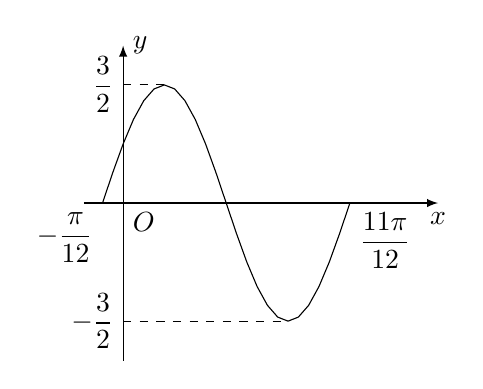
\begin{tikzpicture}[>=latex]
\draw [->] (-0.5,0) -- (4,0) node [below] {$x$};
\draw [->] (0,-2) -- (0,2) node [right] {$y$};
\draw (0,0) node [below right] {$O$};
\draw ({-pi/12},0) node [below left] {$-\dfrac{\pi}{12}$};
\draw ({11*pi/12},0) node [below right] {$\dfrac{11\pi}{12}$};
\draw [domain = {-pi/12}:{11*pi/12}] plot (\x,{1.5*sin(2*\x/pi*180+30)});
\draw [dashed] (0,1.5) -- ({pi/6},1.5) (0,-1.5) -- ({8*pi/12},-1.5);
\draw (0,-1.5) node [left] {$-\dfrac 32$} (0,1.5) node [left] {$\dfrac 32$};
\end{tikzpicture}
\end{center}
\item 写出满足$\tan \alpha=\sqrt 3$的所有$\alpha$的集合.
\item 比较下列各组数的大小, 并说明理由:\\
(1) $\tan (-\dfrac 27\pi )$与$\tan (-\dfrac 25\pi )$;\\
(2) $\cot 231^\circ$与$\cot 237^\circ$;\\
(3) $\tan (k\pi -\dfrac\pi 3)$与$\tan (k\pi +\dfrac\pi 3)$, $k\in \mathbf{Z}$.
\item 求函数$y=\tan (3x+\dfrac\pi 4)$的定义域, 并写出其单调区间. 
\item 指出下列各种量中的向量:\\
(1) 密度;\\
(2) 体积;\\
(3) 速度;\\
(4) 能量;\\
(5) 电阻;\\
(6) 加速度;\\
(7) 功;\\
(8) 力矩.\\
你能找出更多向量的例子吗?
\item 中国象棋中的``马''走``日''. 如图是一个棋盘, 当``马''自点$A$走``一步''后的落点可以为点$A_1$、$A_2$或$A_3$, 表示该``马''走``一步''的向量为$\overrightarrow{AA_1}$、$\overrightarrow{A_A2}$或$\overrightarrow{AA_3}$, 它们是相等的向量吗? 在图中分别用向量表示当``马''在点$B$处各走``一步''的情形.
\begin{center}
\begin{tikzpicture}[>=latex,scale = 0.5]
\foreach \i in {0,1,...,9}
{ \draw (0,\i) -- (8,\i);};
\foreach \i in {0,1,...,8}
{ \draw (\i,0) -- (\i,4) (\i,5) -- (\i,9);};
\draw (0,4) -- (0,5) (8,4) -- (8,5);
\draw (1,4.5) node {\rotatebox{90}{楚}};
\draw (2.3,4.5) node {\rotatebox{90}{河}};
\draw (5.7,4.5) node {\rotatebox{90}{汉}};
\draw (7,4.5) node {\rotatebox{90}{界}};
\draw (3,0) -- (5,2) (5,0) -- (3,2) (3,7) -- (5,9) (5,7) -- (3,9);
\draw [very thin] (0.6,1.9) -- (0.9,1.9) -- (0.9,1.6) (0.6,2.1) -- (0.9,2.1) -- (0.9,2.4) (1.4,1.9) -- (1.1,1.9) -- (1.1,1.6) (1.4,2.1) -- (1.1,2.1) -- (1.1,2.4);
\draw [very thin] (6.6,1.9) -- (6.9,1.9) -- (6.9,1.6) (6.6,2.1) -- (6.9,2.1) -- (6.9,2.4) (7.4,1.9) -- (7.1,1.9) -- (7.1,1.6) (7.4,2.1) -- (7.1,2.1) -- (7.1,2.4);
\draw [very thin] (0.6,6.9) -- (0.9,6.9) -- (0.9,6.6) (0.6,7.1) -- (0.9,7.1) -- (0.9,7.4) (1.4,6.9) -- (1.1,6.9) -- (1.1,6.6) (1.4,7.1) -- (1.1,7.1) -- (1.1,7.4);
\draw [very thin] (6.6,6.9) -- (6.9,6.9) -- (6.9,6.6) (6.6,7.1) -- (6.9,7.1) -- (6.9,7.4) (7.4,6.9) -- (7.1,6.9) -- (7.1,6.6) (7.4,7.1) -- (7.1,7.1) -- (7.1,7.4);
\foreach \i in {0,2,4,6}
{\draw ({\i+0.1},2.6) -- ({\i+0.1},2.9) -- ({\i+0.4},2.9);
\draw ({\i+0.1},3.4) -- ({\i+0.1},3.1) -- ({\i+0.4},3.1);
\draw ({\i+0.1},5.6) -- ({\i+0.1},5.9) -- ({\i+0.4},5.9);
\draw ({\i+0.1},6.4) -- ({\i+0.1},6.1) -- ({\i+0.4},6.1);};
\foreach \i in {0,2,4,6}
{\draw ({8-\i-0.1},2.6) -- ({8-\i-0.1},2.9) -- ({8-\i-0.4},2.9);
\draw ({8-\i-0.1},3.4) -- ({8-\i-0.1},3.1) -- ({8-\i-0.4},3.1);
\draw ({8-\i-0.1},5.6) -- ({8-\i-0.1},5.9) -- ({8-\i-0.4},5.9);
\draw ({8-\i-0.1},6.4) -- ({8-\i-0.1},6.1) -- ({8-\i-0.4},6.1);};
\filldraw [fill = white, draw = black] (1,0) circle (0.5);
\draw (1,0) node {馬} (1,-1) node {$A$};
\filldraw (7,0) circle (0.1) node [below] {$B$};
\filldraw (0,2) circle (0.1) node [left] {$A_1$};
\filldraw (2,2) circle (0.1) node [above right] {$A_2$};
\filldraw (3,1) circle (0.1) node [above right] {$A_3$};
\end{tikzpicture}
\end{center}
\item 如图, 点$O$是正六边形$ABCDEF$的中心, 分别写出图中
\begin{center}
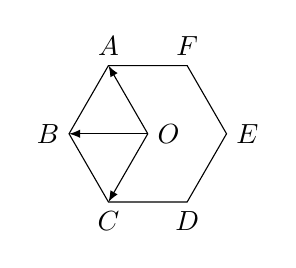
\begin{tikzpicture}[>=latex]
\draw (0,0) node [right] {$O$} coordinate (O);
\draw (60:1) node [above] {$F$} coordinate (F);
\draw (120:1) node [above] {$A$} coordinate (A);
\draw (-1,0) node [left] {$B$} coordinate (B);
\draw (240:1) node [below] {$C$} coordinate (C);
\draw (300:1) node [below] {$D$} coordinate (D);
\draw (1,0) node [right] {$E$} coordinate (E);
\draw (A) -- (B) -- (C) -- (D) -- (E) -- (F) -- cycle;
\draw [->] (O) -- (A);
\draw [->] (O) -- (B);
\draw [->] (O) -- (C);
\end{tikzpicture}
\end{center}
(1) 与$\overrightarrow{OA}$相等的向量;\\
(2) 与$\overrightarrow{OB}$平行的向量;\\
(3) 与$\overrightarrow{OC}$模相等的向量;\\
(4) $\overrightarrow{OB}$的负向量. 
\item 在$\triangle ABC$中, 化简:
(1) $\overrightarrow{AB}-\overrightarrow{AC}=$\blank{50};\\
(2) $\overrightarrow{BC}-\overrightarrow{AC}=$\blank{50}.
\item 已知$A$、$B$、$C$、$D$、$E$是平面上任意五个点, 求证: $\overrightarrow{AE}=\overrightarrow{AB}+\overrightarrow{BC}+\overrightarrow{CD}+\overrightarrow{DE}$. 这个结果可以推广到更多点的情况吗?
\item 试说明, 如果三个首尾相接的向量$\overrightarrow a$、$\overrightarrow b$和$\overrightarrow c$所在的线段能拼接成三角形, 那么一定满足条件$\overrightarrow a+\overrightarrow b+\overrightarrow c=0$. 反过来, 如果$\overrightarrow a+\overrightarrow b+\overrightarrow c=0$, 那么三向量$\overrightarrow a$、$\overrightarrow b$和$\overrightarrow c$所在的线段一定能拼接成三角形吗? 说明理由.
\item 化简下列向量线性运算:\\
(1) $4(2\overrightarrow a-\overrightarrow b)+3(3\overrightarrow a-2\overrightarrow b)$;\\
(2) $\dfrac 14(\overrightarrow a+2\overrightarrow b)-\dfrac 16(5\overrightarrow a-2\overrightarrow b)+\dfrac 14\overrightarrow b$;\\
(3) $2(3\overrightarrow a-4\overrightarrow b+\overrightarrow c)-3(2\overrightarrow a+\overrightarrow b-3\overrightarrow c)$.
\item 根据下列条件, 求向量$\overrightarrow x$:\\
(1) $2\overrightarrow x+3(\overrightarrow b+\overrightarrow x)=0$;\\
(2) $2\overrightarrow a+5(\overrightarrow b-\overrightarrow x)=0$;\\
(3) $\dfrac 13(\overrightarrow x-\overrightarrow a)-\dfrac 12(\overrightarrow b-2\overrightarrow x+\overrightarrow x)+\overrightarrow b=0$.
\item 如图, 在$\triangle ABC$中, 已知$D$是$BC$的中点, $G$是$\triangle ABC$的重心. 设向量$\overrightarrow{BC}=\overrightarrow a$, 向量$\overrightarrow{AC}=\overrightarrow b$. 试用向量$\overrightarrow a$、$\overrightarrow b$分别表示向量$\overrightarrow{AD}$、$\overrightarrow{AG}$、$\overrightarrow{GC}$.
\begin{center}
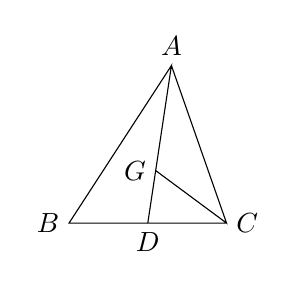
\begin{tikzpicture}[>=latex]
\draw (0,0) node [left] {$B$} coordinate (B);
\draw (2,0) node [right] {$C$} coordinate (C);
\draw (1.3,2) node [above] {$A$} coordinate (A);
\draw ($(B)!0.5!(C)$) node [below] {$D$} coordinate (D);
\draw ($(A)!{2/3}!(D)$) node [left] {$G$} coordinate (G);
\draw (C) -- (B) -- (A) -- (D) (G) -- (C) -- (A);
\end{tikzpicture}
\end{center}
\item 设$\overrightarrow a$、$\overrightarrow b$是两个向量, 其中$\overrightarrow a\ne 0$, $\overrightarrow b$在$\overrightarrow a$方向上的投影是$\overrightarrow {b'}$. 又设$\lambda \in \mathbf{R}$. 分$\lambda \ge 0$与
$\lambda  <0$两种情况, 证明$\lambda \overrightarrow b$在$\overrightarrow a$方向上的投影是$\lambda  \overrightarrow {b'}$.
\item 若$\triangle ABC$为等边三角形, 求下列各角:\\
(1) $\langle \overrightarrow{CA}, \overrightarrow{CB}\rangle$;\\
(2) $\langle \overrightarrow{AC}, \overrightarrow{BC}\rangle$;\\
(3) $\langle \overrightarrow{AB}, \overrightarrow{BC}\rangle$.
\item 已知$|\overrightarrow a|=5$, $|\overrightarrow b|=6$, $\sin \langle \overrightarrow a, \overrightarrow b\rangle =0.6$. 求$\overrightarrow b$在$\overrightarrow a$方向上的投影与数量投影. 
\item 在$\triangle ABC$中, 已知$\overrightarrow{AB}\cdot \overrightarrow{BC}=0$. 判断$\triangle ABC$的形状, 并说明理由.
\item 填空题:\\
(1) 设向量$\overrightarrow a$、$\overrightarrow b$满足$|\overrightarrow a|=4$, $|\overrightarrow b|=9$, $\langle \overrightarrow a, \overrightarrow b\rangle =\dfrac \pi 6$, 则$\overrightarrow a\cdot (\overrightarrow a-\overrightarrow b)=$\blank{50};\\
(2) 设向量$\overrightarrow a$、$\overrightarrow b$满足$|\overrightarrow a|=5$, $|\overrightarrow b|=6$, $(\overrightarrow a+\overrightarrow b)\cdot \overrightarrow b=21$, 则$\langle \overrightarrow a, \overrightarrow b\rangle =$\blank{50}.
\item 设向量$\overrightarrow a$、$\overrightarrow b$满足$|\overrightarrow a|=2$, $|\overrightarrow b|=3$, 且$\langle \overrightarrow a, \overrightarrow b\rangle =120^\circ$. 求$|\overrightarrow a+\overrightarrow b|$.
\item 如图, $\overrightarrow i$与$\overrightarrow j$分别是平面直角坐标系中$x$轴与$y$轴正方向上的单位向量, 点$A$在第一象限内, 与坐标原点$O$的距离为$a$, $\overrightarrow{OA}$与$x$
轴的夹角为$\theta$ . 又设$A'$是$A$关于$x$轴的对称点. 把向量$\overrightarrow{OA}$、$\overrightarrow{OA'}$表
示成向量$\overrightarrow i$与$\overrightarrow j$的线性组合.
\begin{center}
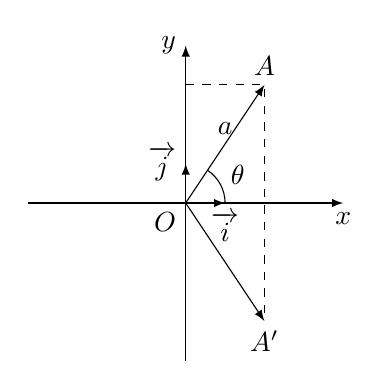
\begin{tikzpicture}[>=latex,scale= 0.5]
\draw [->] (-4,0) -- (4,0) node [below] {$x$} coordinate (x);
\draw [->] (0,-4) -- (0,4) node [left] {$y$};
\draw (0,0) node [below left] {$O$} coordinate (O);
\draw [->] (0,0) -- (1,0) node [below] {$\overrightarrow i$};
\draw [->] (0,0) -- (0,1) node [left] {$\overrightarrow j$};
\draw [->] (0,0) -- (2,3) node [above] {$A$} coordinate (A);
\draw [->] (0,0) -- (2,-3) node [below] {$A'$} coordinate (A1);
\draw [dashed] (0,3) -- (2,3) -- (2,-3);
\draw (1,1.5) node [above] {$a$};
\draw (0,0) pic ["$\theta$",draw,angle eccentricity = 1.5]{angle = x--O--A};
\end{tikzpicture}
\end{center}
\item 已知平行四边形$ABCD$的对角线交于点$O$, 且$\overrightarrow{OA}=\overrightarrow a$, $\overrightarrow{OB}=\overrightarrow b$. 把向量$\overrightarrow{OC}$、$\overrightarrow{OD}$、$\overrightarrow{DC}$与$\overrightarrow{BC}$表示成$\overrightarrow a$与$\overrightarrow b$的线性组合.
\item 设$G$为$\triangle ABC$的重心, 用向量$\overrightarrow{BC}=\overrightarrow a$与$\overrightarrow{AC}=\overrightarrow b$的线性组合来表示向量$\overrightarrow{AG}$、$\overrightarrow{BG}$与$\overrightarrow{CG}$. 
\item 已知向量$\overrightarrow a=(-2, 3)$, $\overrightarrow b=(2, -5)$. 求$3\overrightarrow a-\overrightarrow b$的坐标及$|3\overrightarrow a-\overrightarrow b|$.
\item 求向量$\overrightarrow a=(3, -4)$的单位向量的坐标.
\item 已知平面上$A$、$B$、$C$三点的坐标分别为$(0, 1)$、$(1, 2)$、$(3, 4)$, 求$\overrightarrow{AB}$、$\overrightarrow{BC}$、$\overrightarrow{AC}$的坐标, 并证明$A$、$B$、$C$三点共线.
\item 已知向量$\overrightarrow a=(2, 3)$, $\overrightarrow b=(-2, 4)$, $\overrightarrow c=(-1, -2)$. 求$\overrightarrow a\cdot \overrightarrow b$, $\overrightarrow c\cdot (\overrightarrow a-\overrightarrow b)$.
\item 已知向量$\overrightarrow a=(-3, 4)$, $\overrightarrow b=(5, 12)$. 求$|\overrightarrow a|$、$|\overrightarrow b|$以及$\langle \overrightarrow a, \overrightarrow b\rangle$.
\item 在$\triangle ABC$中, 已知$A$、$B$、$C$三点的坐标分别为$(-2, 3)$、$(0, -1)$、$(1, k)$, 且$\angle C$为直角. 求实数$k$的值.
\item 已知向量$\overrightarrow a=(1, 2)$, $\overrightarrow b=(3, 1)$, $\overrightarrow c=\overrightarrow b-k\overrightarrow a$, 且$\overrightarrow a\perp \overrightarrow c$. 求实数$k$的值及向量$\overrightarrow c$的
坐标.  
\item 已知坐标平面上三个点$A(1, 1)$、$B(4, 2)$与$C(-2, -6)$, 求
$\triangle ABC$的面积.
\item 如图, 已知$\triangle ABC$, $D$、$E$分别是$AB$、$AC$的中点. 求证: $DE\parallel BC$.
\begin{center}
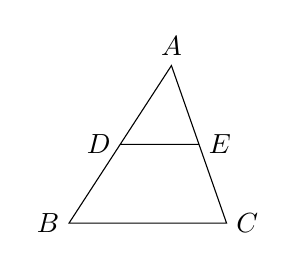
\begin{tikzpicture}[>=latex]
\draw (0,0) node [left] {$B$} coordinate (B);
\draw (2,0) node [right] {$C$} coordinate (C);
\draw (1.3,2) node [above] {$A$} coordinate (A);
\draw ($(A)!0.5!(B)$) node [left] {$D$} coordinate (D);
\draw ($(A)!0.5!(C)$) node [right] {$E$} coordinate (E);
\draw (B) -- (C) -- (A) -- cycle (D) -- (E);
\end{tikzpicture}
\end{center}
\item 已知平面上$A$、$B$两点的坐标分别是$(2, 5)$、$(3, 0)$, $P$是直线$AB$上的一点, 且$\overrightarrow{AP}=-\dfrac 23\overrightarrow{PB}$. 求点$P$的坐标.
\item 已知两个力(单位: $\text{N}$)$\overrightarrow{f_1}$与$\overrightarrow{f_2}$的夹角为$60^\circ$, 其中$\overrightarrow{f_1}=(2, 0)$. 某质点在这两个力的共同作用下, 由点$A(1, 1)$移动至点$B(6, 6)$(单位: \text{m}).\\
(1) 求$\overrightarrow{f_2}$;\\
(2) 求$\overrightarrow{f_1}$与$\overrightarrow{f_2}$的合力对质点所做的功.
\item 已知平面上三点$A$、$B$、$C$的坐标分别是$(1, 7)$、$(2, 2)$、$(0, 1)$, $P$为直线$AC$上的一动点. 问: $P$在什么位置时, $|\overrightarrow{BP}|$取到最小值?
\item 已知$(x+2y)+(5x-y)\mathrm{i}=9+\mathrm{i}$, 其中$x$、$y\in \mathbf{R}$. 求$x$、$y$的值.
\item 计算:\\
(1) $(-1+3\mathrm{i})+(2+6\mathrm{i})$;\\
(2) $(3-2\mathrm{i})-(4+\mathrm{i})$;\\
(3) $(\dfrac 12-\dfrac{\sqrt 3}2\mathrm{i})(\sqrt 3+\mathrm{i})$;\\
(4) $(1+\mathrm{i})^6$;\\
(5) $\dfrac2{1-\mathrm{i}}$;\\
(6) $\dfrac{-1+2\mathrm{i}}{-1-2\mathrm{i}}$.
\item 对复数$z_1$、$z_2\in \mathbf{C}$, 验证: $\overline{z_1+z_2}=\overline{z_1}+\overline{z_2}$, $\overline{z_1-z_2}=\overline{z_1}0-\overline{z_2}$.
\item 在下列复数中, 哪些是实数?  哪些是虚数?  哪些是纯虚数?  各数的实部和虚部分别是什么?\\
$-5+6\mathrm{i}$、$\dfrac{\sqrt 2}2+\dfrac{\sqrt 2}2\mathrm{i}$、$-\sqrt 3$、$\mathrm{i}$、$0$、$\cos \dfrac\pi 5+\mathrm{i}\sin\dfrac\pi 5$.
\item 下列关于复数$z$和$\overline z$的命题是真命题还是假命题? 请给出结论并说明理由.\\
(1) $z+\overline z$一定是实数;\\
(2) $z-\overline z$一定是纯虚数;\\
(3) $若z-\overline z=0$, 则$z$是实数;\\
(4) 若$z+\overline z=0$, 则z是纯虚数.
\item 求实数$m$的值或取值范围, 使得复数$z=(m+2)+(m-1)\mathrm{i}$分别是:\\
(1) 实数;\\
(2) 虚数;\\
(3) 纯虚数. 
\item 当复数$z$满足下列条件时, 分别指出$z$在复平面上所对应的点$Z$的位置:\\
(1) $z$是正实数;\\
(2) $z$是负实数;\\
(3) $z$是实部小于零、虚部大于零的虚数;\\
(4) $z$是虚部小于零的纯虚数.
\item 如果复数$z=(m-2)+(m^2-16)\mathrm{i}$($m\in \mathbf{R}$)在复平面上所对应的点在第四象限, 求$m$的取值范围.
\item 设复数$3-4\mathrm{i}与5-6\mathrm{i}$在复平面上所对应的向量分别为$\overrightarrow{OA}$与$\overrightarrow{OB}$($O$为坐标原点), 求向量$\overrightarrow{AB}$及$\overrightarrow{BA}$所对应的复数.
\item 已知复平面上有点$C(2, 4)$和点$D$, 使得向量$CD$所对应的复数是$-3-\mathrm{i}$. 求点$D$的坐标.
\item 计算下列复数的模:\\
(1) $(4-3\mathrm{i})+(-12-5\mathrm{i})$;\\
(2) $(2-\sqrt 3\mathrm{i})(\sqrt 6-\mathrm{i})^2$;\\
(3) $\dfrac{7+\mathrm{i}}{(3-4\mathrm{i})^2}$.
\item 设复数$z_1=6+8\mathrm{i}$与$z_2=9-4\mathrm{i}$在复平面上所对应的点为$Z_1$与$Z_2$, 试指出$Z_1$、$Z_2$与以原点为圆心、$10$为半径的圆$C$的位置关系.
\item 设复平面上平行四边形$OMNP$的顶点$O$、$M$、$P$的坐标分别为$(0, 0)$、$(3, 4)$、$(-2, -3)$, 求$ON$的长度.
\item 求复数$8+5\mathrm{i}$与$4-2\mathrm{i}$在复平面上所对应的点之间的距离. 
\item 已知$k$是一个实常数, 而关于$x$的一元二次方程$x^2-2kx-k=0$有两个虚根. 求$k$的取值范围.
\item 在复数范围内解方程:\\
(1) $x^2+2=0$;\\
(2) $x^2+2x+3=0$;\\
(3) $2(x^2+4)=5x$.
\item 若$x_1$和$x_2$是方程$2x^2+x+3=0$的两个根, 求$\dfrac 1{x_1}+\dfrac1{x_2}$的值.
\item 下列复数是否用三角形式来表示的? 为什么?\\
(1) $3\pi (\cos 0.5+\mathrm{i}\sin 0.5)$;\\
(2) $2(\sin 1+\mathrm{i}\cos 1)$;\\
(3) $\cos 131\pi +\mathrm{i}\sin 131\pi$;\\
(4) $\sqrt 2(\cos 0.3\pi +\mathrm{i}\sin 0.2\pi)$;\\
(5) $-2(\cos \dfrac \pi 4+\mathrm{i}\sin\dfrac \pi 4)$;\\
(6) $3(\cos \dfrac\pi 5-\mathrm{i}\sin\dfrac \pi 5)$.
\item 把下列复数用三角形式表示(用辐角主值):\\
(1) $3$;\\
(2) $-2\mathrm{i}$;\\
(3) $1+\mathrm{i}$;\\
(4) $-1+\sqrt 3\mathrm{i}$.
\item 计算:\\
(1) $8(\cos \dfrac\pi 6+\mathrm{i}\sin \dfrac\pi 6)\cdot 2(\cos \dfrac\pi 3+\mathrm{i}\sin\dfrac \pi 3)$;\\
(2) $\dfrac{6(\cos \dfrac{3\pi} 5+\mathrm{i}\sin \dfrac{3\pi} 5)}{2(\cos \dfrac\pi {10}+\mathrm{i}\sin \dfrac\pi {10})}$;\\
(3) $\sqrt 2(\cos \dfrac\pi 6+\mathrm{i}\sin \dfrac\pi 6)$.
\item 求$1$的所有四次方根. 
\end{enumerate}

\end{document}
